\documentclass[11pt]{article}
\usepackage[margin=1in]{geometry}
\usepackage{amsmath,amssymb,amsthm}
\usepackage{enumitem}
\usepackage{tikz}
\usetikzlibrary{positioning,arrows.meta,calc}
\usepackage[backend=biber,style=apa,natbib]{biblatex}
\addbibresource{problem.bib}
\usepackage{hyperref}
\usepackage{xcolor}
\hypersetup{colorlinks=true,linkcolor=blue!50!black,urlcolor=blue!50!black,citecolor=blue!50!black}

\newtheorem{definition}{Definition}
\newtheorem{problem}{Problem}
\newtheorem{claim}{Claim}
\newtheorem{remark}{Remark}
\newtheorem{proposition}{Proposition}

\title{Cost-Bounded Program Synthesis as a Model of\\
       Arithmetic Strategy Acquisition}
\author{Statement of the mathematical problem\\
\small T.\ Savich, Indiana University}
\date{\today}

\begin{document}
\maketitle

\noindent\fbox{\parbox{\textwidth}{\small\textbf{Status:} Working
document, not a publication-ready paper. The framework borrows
vocabulary from Brandom and Lakoff--N\'u\~nez; specific
formalizations (e.g.\ the cost functor, the metaphor labelling)
are proposals to be tested against primary sources and empirical
evidence, not proved structure. Treat all formal claims as
conjectural unless explicitly proved. The companion documents in
\texttt{\textasciitilde{}/Desktop/Best\_Day/PML/} are ground truth
for what is and is not defensible in this project's appropriation
of Brandom and Carspecken; see
\texttt{pml\_existing\_vs\_brandom\_synthesis\_contrast.md} for the
applicable critique.}}
\bigskip

\begin{abstract}
We formulate the discovery of arithmetic strategies and the prediction
of structured misconceptions as a problem in cost-bounded program
synthesis over typed cognitive primitives, under agent-level resource
constraints. A learner is characterized by a working-memory bound, a
facts cache, and a curricularly-determined subset of metaphor-coherent
primitives. The cost of a candidate program depends on the input on
which it is executed; the productive strategy for a learner on an input
is the cost-minimal program in their accessible vocabulary that returns
the target value; misconceptions are cost-competitive
metaphor-coherent programs that return wrong values. The framework
unifies and extends three pre-existing research lineages — Brown and
VanLehn's repair theory of procedural bugs, Siegler's strategy-choice
theory, and the bounded-utility-maximization tradition of computational
rationality — by adding two structural moves: metaphor coherence as the
filter that separates misconceptions from unstructured error, and
base-parameterization of primitives. The latter, viewed
category-theoretically, makes strategic invariance under base-shifts a
theorem under a naturality condition on the cost function rather than a
hypothesis requiring empirical confirmation. What remains for
computation and for empirical study is the mapping of input regimes to
their cost-optimal strategies and applicable misconceptions — the
\emph{topology of arithmetic action}. The problem is well-posed for
simulation; closed-form characterization of optimal programs is not
expected.
\end{abstract}

\section{Introduction}

This document is a problem statement, not a results paper. We
articulate the mathematical object underlying an ongoing computational
project on the structure of K--12 arithmetic strategies and
misconceptions. The intent is to make the problem portable: any reader
engaging with it mathematically should be able to do so without reading
the prototype source.

The empirical anchor of the project is a forty-year tradition of
classroom research that has catalogued hundreds of specific
arithmetic-error patterns. That literature is enormous and
descriptive: it says \emph{we saw this happen}. What it does not say
is \emph{when} a given error will happen, \emph{which problems
trigger it}, or \emph{how to tell in advance} whether a given child is
at risk of making it on a specific problem. A teacher looking at
$23 + 18$ has no operational way to ask: ``of the documented
misconceptions, which ones can possibly manifest on \emph{this}
problem, with \emph{these} numbers?'' The framework below is an
attempt to make that question well-defined.

The central object is a learner who, given an arithmetic input,
attempts to compute a target value by composing primitive cognitive
operations. Strategies are programs the learner produces;
misconceptions are programs the learner produces that fail to match
the target on some inputs. We claim that strategy invention is driven
by cost-minimization under bounded resources, that misconceptions are
structurally cost-competitive programs distinguished from strategies
by metaphor coherence and output correctness, and that the resulting
search problem admits empirically interesting answers but does not in
general admit closed-form ones.

This is not a new problem. Repair theory \parencite{brownvanlehn1980,
vanlehn1990} generates procedural bugs in subtraction from primitives
by applying deletion operations to incomplete procedures and running a
constrained problem-solver. Strategy choice theory and SCADS
\parencite{siegler1988, shragerSiegler1998} simulate children's
strategy discovery. \textcite{young2000} explicitly frames children's
addition strategies as cost-minimizing under a least-effort principle,
reducing predicted error by $63\%$ in a sample of grade-one learners.
\textcite{guhe2011blending, guhe2009commutativity} have formalized
Lakoff and N\'u\~nez's grounding metaphors computationally using
heuristic-driven theory projection and conceptual blending.
\textcite{lewis2014} articulate the abstract framework of which our
problem is a special case: theories are specified as optimal program
problems defined by an adaptation environment, a bounded machine, and
a utility function.

Our contribution is therefore not a new framework but a specific
integration with two structural additions:
\begin{enumerate}[noitemsep,topsep=2pt]
  \item \textbf{Metaphor coherence as the filter on the deformation
        set}: a candidate misconception must instantiate a
        recognizable grounding metaphor. Without this filter the
        cost-competitive-wrong-program set is empirically
        uninformative.
  \item \textbf{Base-parameterization of primitives}: primitives carry
        the working base as a parameter $\sigma_b$, and the cost
        function depends only on structural features (residues modulo
        $b$, absolute cognitive constants). Under this naturality
        condition, strategic invariance under base-shifts is a theorem
        rather than an empirical hypothesis, and computation is
        redirected to questions that genuinely require it: the
        mapping of input regimes to cost-optimal strategies, and the
        applicability boundaries of documented misconceptions.
\end{enumerate}

The setup is intentionally minimal. It is not a theory of cognition.
It is a mathematical object that captures enough structure to be tested
against the empirical literature on documented strategies and
misconceptions, and to predict new ones.

\section{Primitives, programs, semantics}

\begin{definition}[Signature]
A \emph{primitive signature} is a finite set $\Sigma = \{\sigma_1,
\sigma_2, \dots, \sigma_n\}$ with arity and type information for each
$\sigma_i$. Each primitive denotes a total or partial function on a
common semantic universe $U \subseteq \mathbb{Z}^k$. Primitives are
\emph{base-parametric}: where semantics depends on a working base
$b \in \mathbb{N}_{\ge 2}$, the base appears explicitly as a parameter
$\sigma_b$.
\end{definition}

Representative primitives in the prototype include
$\mathrm{iter\_succ}: U \times \mathbb{N} \to U$ (repeated successor),
$\mathrm{iter\_pred}$ (repeated predecessor),
$\mathrm{delta\_to\_next\_base}_b: U \to \mathbb{N}$ (distance from
$x$ to the next non-negative multiple of $b$), and fact-retrieval
primitives. The signature is open: new primitives are added as new
cognitive moves are formalized, and base-specific primitives are
written $\sigma_b$ rather than collapsing to base $10$.

\begin{definition}[Grammar of programs]
Let $\mathcal{G}_\Sigma$ be a context-free grammar generating
sequential compositions over $\Sigma$, with explicit variable binding.
A \emph{program} is a finite term $P \in \mathcal{L}(\mathcal{G}_\Sigma)$
consisting of an ordered list of steps $\langle s_1, \dots, s_d \rangle$
where each step $s_j = (\sigma_{i_j}, \bar{a}_j)$ names a primitive
together with argument references. An argument reference is either an
input index or an earlier step's output. We write
$\mathrm{depth}(P) = d$.
\end{definition}

A program is executed on an input tuple $\bar{x} \in U^m$ by binding
inputs, evaluating each step in sequence, and returning the last
step's output. Execution may fail if a primitive is partial and its
preconditions are violated. We write $P(\bar{x}) \in U \cup \{\bot\}$
for the result.

\begin{remark}
The grammar is restricted to straight-line sequential composition.
Conditional branching and unbounded recursion are deferred. The
twenty-five student-invented strategies catalogued in the project's
prior Python prototype (now subsumed by the present work) are
implementable as register machines and bounded pushdown automata over
this restricted grammar.
\end{remark}

\section{Cost as cognitive load}

\begin{definition}[Cost function]
A \emph{cost function} for a signature $\Sigma$ is a partial map
\[
c : \mathcal{L}(\mathcal{G}_\Sigma) \times U^m \to \mathbb{N} \cup \{\infty\}
\]
that assigns a non-negative integer (or $\infty$, for failing programs)
to each (program, input) pair. Cost decomposes by steps:
\[
c(P, \bar{x}) = \sum_{j=1}^{\mathrm{depth}(P)} c_\sigma(\sigma_{i_j},
\bar{v}_j),
\]
where $\bar{v}_j$ is the resolved argument tuple of step $j$ and
$c_\sigma:\Sigma \times U^* \to \mathbb{N}$ is the per-step cost.
\end{definition}

Cost is \emph{input-dependent}: the same program incurs different cost
on different inputs because primitives such as $\mathrm{iter\_succ}(s,n)$
are linear in $n$ except when $n$ is base-aligned, in which case the
operation is treated as a single chunked move at unit cost. The exact
per-step cost function is part of the model and is empirically
calibrated; it is not a free choice.

\begin{definition}[Structurally defined cost]
\label{def:structural-cost}
A cost function $c$ is \emph{structurally defined} (with respect to
base $b$) if $c_\sigma$ depends only on: residues $x \bmod b$ of its
numeric arguments; absolute cognitive constants (e.g.\ a subitization
bound); and the structural form of the primitive itself. Cost
functions that mention numeric literals tied to a specific base — for
example a clause that fires only when $n \bmod 10 = 0$ — are
\emph{not} structurally defined.
\end{definition}

\noindent The prototype's current cost function is \emph{not}
structurally defined; converting it to a structural form is the first
implementation task and is what makes the invariance claim of
\S\ref{sec:algebra} a theorem.

\section{Learner profiles}

\begin{definition}[Learner profile]
A \emph{learner profile} is a triple
\[
\ell = (b_w, F, E),
\]
where $b_w \in \mathbb{N}$ is the \emph{working-memory bound} (maximum
program depth the learner will compose); $F \subseteq U^m \times U$ is
the \emph{facts cache} (input-output pairs available at near-zero
cost); and $E \subseteq \Pi$ is the \emph{metaphor exposure} (the
subset of grounding metaphors the learner has encountered through
curriculum). $\Pi$ is the set of grounding metaphor labels
(\S\ref{sec:metaphor}). The learner's accessible primitives are
\[
\Sigma_E = \{\sigma \in \Sigma : \mu(\sigma) \cap E \ne \emptyset\},
\]
where $\mu:\Sigma \to 2^{\Pi}$ is the metaphor labelling of primitives.
\end{definition}

\begin{remark}
The profile records a single learner at a single point in time. For
example, $\text{Tommy} = (5,\ \{(9,1)\mapsto 10,\ (8,2)\mapsto 10,\
(7,3)\mapsto 10\},\ E_{\mathrm{IM-K}})$ asserts that Tommy will compose
programs of depth at most $5$, has memorized the partitions of $10$
involving one-digit complements, and has been exposed to the metaphor
set $E_{\mathrm{IM-K}}$ instantiated by Illustrative Mathematics
Kindergarten. Different learners are different points in profile
space; learning is a trajectory through that space.
\end{remark}

\section{The two synthesis problems}

For a fixed target function $f:I \to U$ (where $I \subseteq U^m$ is a
bounded input space; see \S\ref{sec:input-space}) and a learner profile
$\ell = (b_w, F, E)$:

\begin{problem}[Productive synthesis]
\label{prob:productive}
For each $\bar{x} \in I$, find
\[
P^*(\ell, \bar{x}) \in \arg\min \big\{ c(P, \bar{x}) :
P \in \mathcal{L}(\mathcal{G}_{\Sigma_E}),\
\mathrm{depth}(P) \le b_w,\ P(\bar{x}) = f(\bar{x}) \big\}.
\]
\end{problem}

\begin{problem}[Deformation synthesis]
\label{prob:deformation}
With $C^* = c(P^*(\ell, \bar{x}), \bar{x})$, find
\[
D(\ell, \bar{x}) = \big\{ P \in \mathcal{L}(\mathcal{G}_{\Sigma_E}) :
\mathrm{depth}(P) \le b_w,\ c(P, \bar{x}) \le C^*,\ P(\bar{x}) \ne
f(\bar{x}),\ P\ \text{is metaphor-coherent} \big\}.
\]
\end{problem}

The metaphor-coherence requirement is defined in
\S\ref{sec:metaphor}. Without it, $D(\ell, \bar{x})$ contains an
intractable number of structurally meaningless cost-competitive
programs.

\section{Metaphor as a constraint}
\label{sec:metaphor}

\begin{definition}[Metaphor labelling and coherence]
Let $\Pi = \{\pi_{OC}, \pi_{OBJ}, \pi_{MS}, \pi_{MAP}\}$ be the set of
the four Lakoff--N\'u\~nez grounding metaphors for arithmetic:
\emph{Object Collection}, \emph{Object Construction},
\emph{Measuring Stick}, and \emph{Motion Along a Path}
\parencite{lakoffNunez2000}. Each primitive carries a non-empty set of
compatible metaphor labels: $\mu:\Sigma \to 2^\Pi \setminus
\{\emptyset\}$. A program $P = \langle s_1, \dots, s_d \rangle$ is
\emph{metaphor-coherent} if there exists at least one label
$\pi \in \Pi$ such that $\pi \in \mu(\sigma_{i_j})$ for all $j$;
equivalently, $\bigcap_{j=1}^{d} \mu(\sigma_{i_j}) \ne \emptyset$.
\end{definition}

A program is metaphor-coherent iff some single metaphor admits every
primitive it uses. A blend is permitted at the metaphor level (a
primitive may carry multiple labels), not by composing primitives
across incompatible metaphors within a single program.

\begin{remark}[Inferential structure transferred]
\parencite{lakoffNunez2000}: Object Collection transfers magnitude,
closure for addition, and the equational laws via grouping and
pooling; it breaks at zero (requiring the \emph{Zero Collection
Metaphor} as a repair) and for negative and fractional quantities.
Object Construction extends Object Collection with part--whole
decomposition; its repair at zero is the \emph{Zero Object Metaphor}.
Measuring Stick maps continuous unit-length segments end-to-end,
breaks at zero, and does not naturally extend to negatives. Motion
Along a Path is unique in that it does \emph{not} break at zero or
negatives but requires the \emph{Rotation by 180\textdegree\ Is
Multiplication by $-1$} blend to handle multiplication by negatives.
Fractions are not the target of a separate grounding metaphor: they
emerge by stretching Object Construction, Measuring Stick, and Motion
Along a Path internally, since Object Collection cannot conceptualize
fractional collections.
\end{remark}

\begin{remark}[Metaphor as curriculum, not metaphor as truth]
The framework does not claim that metaphors are mental facts. It
claims that primitives factor into structural families that may be
selectively available to a learner, and that programs composed across
families are not what learners actually invent. The labelling $\mu$ is
a hypothesis to be empirically tested. Existing computational
implementations of L\&N metaphors using heuristic-driven theory
projection \parencite{guhe2011blending, guhe2009commutativity} can
supply candidate labellings.
\end{remark}

\section{Error and misconception}
\label{sec:error}

\begin{definition}[Error]
An \emph{error} is a single-instance deviation from the intended
program. The learner intended to execute $P$ but produced
$P'(\bar{x}) \ne P(\bar{x})$. Errors are not stable; the learner would
not reliably reproduce them. The set of possible errors is
unconstrained.
\end{definition}

\begin{definition}[Misconception]
A \emph{misconception} for learner $\ell$ on input regime $R \subseteq
I$ is a metaphor-coherent program $P' \in D(\ell, \bar{x})$ such that:
\begin{enumerate}[noitemsep,topsep=2pt,label=(M\arabic*)]
  \item $c(P', \bar{x}) \le c(P^*(\ell, \bar{x}), \bar{x})$ for all
        $\bar{x} \in R$ (cost-competitive across the regime);
  \item $P'(\bar{x}) \ne f(\bar{x})$ for some non-empty subset of $R$
        (the strategy is wrong somewhere in its regime).
\end{enumerate}
\end{definition}

\begin{remark}
The framework cannot predict individual errors and does not try to.
The set of possible errors is unbounded; the set of misconceptions is
constrained by metaphor coherence and cost-competitiveness. This is the
deliberate trade-off.
\end{remark}

\begin{remark}[Overgeneralization]
A common shape of misconception is the over-application of a strategy
outside its regime of correctness. Let
\[
R(P) = \{\bar{x} \in I : P(\bar{x}) = f(\bar{x}) \ \text{and}\
P \in \arg\min_{Q} c(Q, \bar{x}) \text{ with } Q\ \text{correct}\}.
\]
A learner whose curricular input distribution sampled only $R(P)$ and
who has not learned a boundary detector treats $P$ as universally
applicable, running $P$ on $\bar{x} \in I \setminus R(P)$ and
producing $P(\bar{x}) \ne f(\bar{x})$. The misconception is induced by
the curriculum, not by the individual. This is the mathematical
content of \textcite{masonStephensWatson2009}'s observation that
``students need to know the direction in which compensation has to be
carried out in order to maintain equivalence.''
\end{remark}

\section{Input space}\label{sec:input-space}

\begin{definition}[Structured input regime]
The input space $I$ is bounded: $I \subseteq \{(\bar{x}) \in U^m :
\|\bar{x}\|_\infty \le N\}$ for some chosen $N$. Within this box, the
relevant structure is the distance of each coordinate from a
base-aligned value:
$\delta_b(x) = \min_k |x - k\cdot b|$.
Strategies that exploit base-alignment have distinct cost profiles for
inputs of small $\delta_b$ versus large $\delta_b$.
\end{definition}

The mathematically interesting subset of $I$ is $I$ quotiented by the
equivalence
\[
\bar{x} \sim_b \bar{x}' \iff (\delta_b(x_1), \delta_b(x_2), \dots)
= (\delta_b(x'_1), \delta_b(x'_2), \dots).
\]
On each equivalence class, the cost-optimal program is constant. The
full input space need not be searched; one representative per
equivalence class suffices for structural results.

\section{Fractions as recursive units coordination}
\label{sec:fractions}

The whole-number formulation extends to fractions by a structural
analogy.

\begin{claim}[The unit-of-units shift]
Fractional reasoning is the same problem with the unit-axis shifted.
Where whole-number strategies exploit the relation between a number
$n$ and the base $b$ (via $\delta_b(n)$), fractional strategies
exploit the relation between a fraction $m/n$ and a recursive
partition of a unit of units. Specifically, $1/n$ acts as the basic
multiplicative unit of a \emph{splitting world} that stands in
operational isomorphism to the \emph{counting world} whose basic unit
is the successor of $1$ \parencite{confreySmith1995}.
\end{claim}

\textcite{olive1999} characterises the development of fractional
schemes as a reorganisation of whole-number generalised number
sequences ``inwards'' — producing ``units within units within a
unit'' — and frames this as a recursive division analogous in
structure to the outward exponential structure of whole-number bases.
\textcite{izsak2008} define recursive partitioning as ``taking a
partition of a partition in the service of a non-partitioning goal''
and require the learner to construct ``a unit of units of units'' for
fraction multiplication. The Steffe--Hackenberg--Norton tradition
\parencite{steffeOlive2010, hackenberg2007, norton2012splitting} has
established empirically that the number of levels of units a learner
can interiorise predicts which fraction schemes they can construct.

\begin{definition}[Multiplicative concept]
A learner's \emph{multiplicative concept} $MC \in \{1, 2, 3\}$ is the
number of nested unit-levels they can take as given prior to activity.
For each $MC$ level there is a corresponding set of accessible
fraction schemes; we take this hierarchy as constraining the learner's
$\Sigma_E$ when the target $f$ involves fractions.
\end{definition}

\section{An algebraic view}
\label{sec:algebra}

The formulation above is naturally categorical. Make it so explicitly
and a key claim becomes a theorem rather than a hypothesis.

Let $\mathbf{Free}(\Sigma)$ denote the free category generated by
$\Sigma$ under the grammar $\mathcal{G}_\Sigma$. Objects are typed
arities; morphisms are programs; composition is sequential
composition. The semantic interpretation is a functor
\[
\llbracket - \rrbracket : \mathbf{Free}(\Sigma) \longrightarrow
\mathbf{Set}
\]
mapping programs to the functions they compute. The cost function
factors through the monoid $(\mathbb{N}, +, 0)$ via a graded functor
\[
c : \mathbf{Free}(\Sigma) \times I \longrightarrow (\mathbb{N}, +).
\]
The productive synthesis problem (Problem~\ref{prob:productive}) is
then a search for the cost-minimal morphism in the fibre
$\llbracket - \rrbracket^{-1}(f|_{\bar{x}})$. Misconceptions are
cost-bounded morphisms in the complement
$\llbracket - \rrbracket^{-1}(U \setminus \{f(\bar{x})\})$ that
additionally factor through the sub-category generated by the
metaphor-coherent primitives.

For each base $b$ there is a functor instance $c_b$ and a primitive
signature $\Sigma_b$. Base shift is a family of functors
$\Phi_{b \to b'} : \mathbf{Free}(\Sigma_b) \to
\mathbf{Free}(\Sigma_{b'})$ that renames base-specific constants.

\begin{proposition}[Invariance under naturality]
\label{prop:naturality}
If the cost function is structurally defined
(Definition~\ref{def:structural-cost}), then $c$ is natural in $b$:
for every base shift $\Phi_{b \to b'}$ and every program $P$ over
$\Sigma_b$,
\[
c_b(P, \bar{x}) = c_{b'}(\Phi_{b \to b'}(P), \Phi_{b \to b'}(\bar{x})).
\]
Consequently the cost-minimal program shape commutes with base shift:
\[
P^*(\ell, \Phi_{b \to b'}(\bar{x})) \cong \Phi_{b \to b'}(P^*(\ell,
\bar{x})).
\]
\end{proposition}

\begin{proof}[Proof sketch]
By Definition~\ref{def:structural-cost}, $c_\sigma$ depends only on
residues modulo $b$ and absolute cognitive constants. The base shift
$\Phi_{b \to b'}$ preserves both: residues are preserved by
construction (the shift maps $k \cdot b + r$ to $k \cdot b' + r$); the
constants are absolute. Hence $c_b(P, \bar{x}) = c_{b'}(\Phi(P),
\Phi(\bar{x}))$ step by step, and the argmin preserves shape.
\end{proof}

\begin{remark}[What this changes]
Strategic invariance under base shift, written as
Claim~\ref{prop:naturality}, becomes a theorem provable on paper
under the structural-cost condition. Earlier drafts of this paper
proposed an empirical test under bases $\{5, 10, 12\}$ to confirm
invariance. That test is redundant if the cost function is genuinely
structural. What the test \emph{would} reveal, if invariance failed,
is that the cost function is not structural — that some clause is
silently base-specific. That is a useful diagnostic, but not the
research program. The research program is what
Section~\ref{sec:topology} describes.
\end{remark}

\section{The topology of arithmetic action}
\label{sec:topology}

Once invariance is settled by Proposition~\ref{prop:naturality}, the
computationally interesting question is sharper: for a given
$(\Sigma, c, \mu, \ell)$, what does the function
$\bar{x} \mapsto P^*(\ell, \bar{x})$ look like as $\bar{x}$ ranges
over $I$? Which input regimes select which cost-optimal programs?
Which regimes admit which misconceptions?

Call this map the \emph{strategy-applicability map}, $S_\ell : I \to
\mathcal{L}(\mathcal{G}_{\Sigma_E})$, and the corresponding
deformation map $D_\ell : I \to 2^{\mathcal{L}(\mathcal{G}_{\Sigma_E})}$.
Both partition $I$ into level sets — connected regions on which a
single program is cost-optimal or a single deformation is
cost-admissible. The collection of level sets and their boundaries is
what we mean by the \emph{topology of arithmetic action}: a
mathematical-pedagogical structure that says where each strategy and
each misconception is operative as a function of input.

This topology is not derivable in closed form. It is a finite but
combinatorial object whose shape depends on the cost function and the
primitive set in ways that resist symbolic enumeration. Computing it
empirically — over equivalence classes under $\sim_b$, across
operations and curricular profiles — is what the synthesis pipeline
exists to do.

\paragraph{Figure (schematic).}
For the subtraction operation in base $10$ over inputs $(a, b) \in
[0, 100]^2$, the strategy-applicability map partitions the input
square into several regions (Figure~\ref{fig:topology}). When
$\delta_{10}(b)$ is small (the subtrahend is near a base-aligned
value), the make-base strategy is cost-optimal and the
wrong-direction-compensation deformation is cost-admissible. When
$b$ is small absolutely, count-back is cost-optimal and no
make-base-specific deformation can manifest. Elsewhere, naive
$\mathrm{iter\_pred}$ is cost-optimal. The boundaries are where the
cost-optimal program changes; teaching at boundaries is teaching at
the points of productive friction.

\begin{figure}[t]
\centering
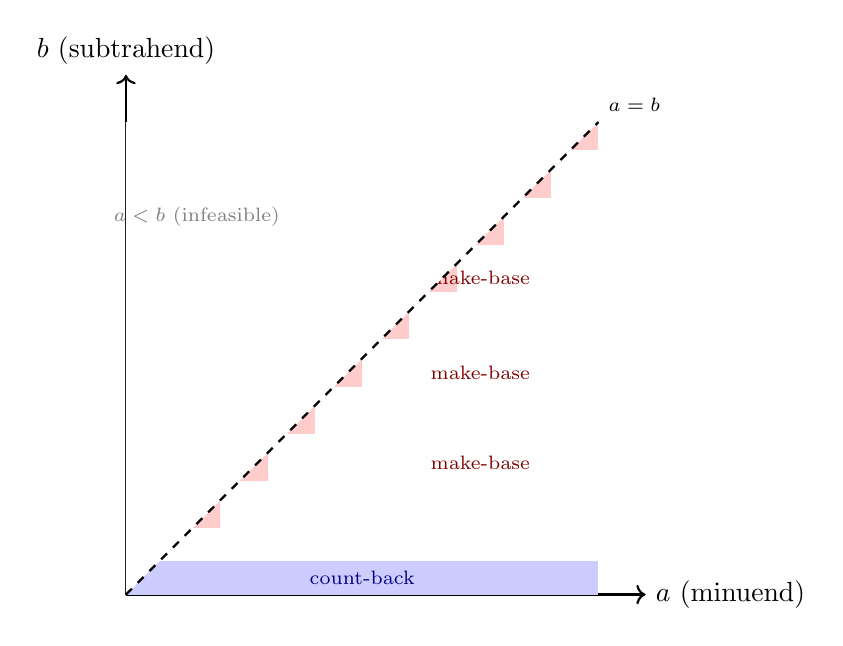
\begin{tikzpicture}[scale=0.06]
  % Axes
  \draw[->, thick] (0,0) -- (110,0) node[right] {$a$ (minuend)};
  \draw[->, thick] (0,0) -- (0,110) node[above] {$b$ (subtrahend)};
  % Region 1: count-back when b small
  \fill[blue!20] (0,0) -- (100,0) -- (100,7) -- (0,7) -- cycle;
  \node[blue!50!black] at (50,3.5) {\scriptsize count-back};
  % Region 2: make-base near multiples of 10
  \foreach \y in {17, 27, 37, 47, 57, 67, 77, 87, 97} {
    \fill[red!20] (\y - 7, \y - 3) rectangle (\y + 3, \y + 3);
  }
  \foreach \y in {28, 47, 67, 86} {
    \node[red!50!black] at (75, \y) {\scriptsize make-base};
  }
  % Region 3: naive iter_pred elsewhere
  \node[gray] at (30,60) {\scriptsize naive iter\_pred};
  \node[gray] at (70,90) {\scriptsize naive iter\_pred};
  % Diagonal: a < b is infeasible
  \fill[white] (0,0) -- (100,100) -- (0,100) -- cycle;
  \draw[dashed, thick] (0,0) -- (100,100) node[above right] {\scriptsize $a = b$};
  \node[gray] at (15,80) {\scriptsize $a < b$ (infeasible)};
\end{tikzpicture}
\caption{Schematic strategy-applicability map for subtraction in base
$10$. Blue: count-back is cost-optimal. Red: make-base is cost-optimal.
Gray: naive repeated decrement is cost-optimal. Boundaries are where
the cost-optimal program changes. Each region also carries its
admissible deformations (not shown).}
\label{fig:topology}
\end{figure}

\paragraph{Empirical content.} Prior work in the project (the
trace-amplification runs on the Big Red HPC) confirms the conditional
character of misconceptions empirically: of forty productive /
deformation pairs tested on amplified input grids, fourteen showed
deformations that fire only under specific input conditions —
$\mathrm{crosses\_base\_ten\_sum} = \mathrm{True}$ for carry-related
addition deformations, $\mathrm{requires\_borrow} = \mathrm{True}$ for
the corresponding subtraction deformations, $\mathrm{left\_has\_zero\_
column} = \mathrm{True}$ for the borrow-with-zero family. Three
structural clusters emerged in the data: four addition deformations
sharing the carry condition, three division deformations sharing the
equal-operand condition, two subtraction deformations sharing the
borrow-with-zero conjunction. These findings are samples of the
topology; characterising it across operations, bases, and curricular
profiles is what synthesis at scale will produce.

\section{Categorical structure: a diagram}

The categorical view collects the main objects in a single commutative
diagram.

\begin{figure}[t]
\centering
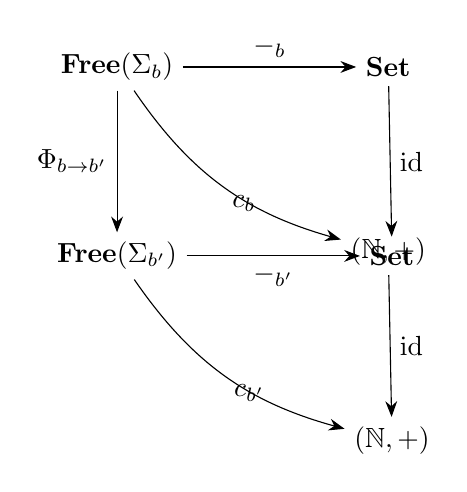
\begin{tikzpicture}[
  node distance = 18mm and 22mm,
  every node/.style = {align=center},
  >={Stealth[length=2mm]}
]
  \node (free) {$\mathbf{Free}(\Sigma_b)$};
  \node[right = of free] (set) {$\mathbf{Set}$};
  \node[below = of free] (free2) {$\mathbf{Free}(\Sigma_{b'})$};
  \node[right = of free2] (set2) {$\mathbf{Set}$};
  \node[below = of set] (nat) {$(\mathbb{N},+)$};
  \node[below = of set2] (nat2) {$(\mathbb{N},+)$};

  \draw[->] (free) -- node[above]{$\llbracket - \rrbracket_b$} (set);
  \draw[->] (free2) -- node[below]{$\llbracket - \rrbracket_{b'}$} (set2);
  \draw[->] (free) -- node[left]{$\Phi_{b\to b'}$} (free2);
  \draw[->] (set) -- node[right]{$\mathrm{id}$} (set2);
  \draw[->] (free) to[bend right=20] node[below right]{$c_b$} (nat);
  \draw[->] (free2) to[bend right=20] node[below right]{$c_{b'}$} (nat2);
  \draw[->] (nat) -- node[right]{$\mathrm{id}$} (nat2);
\end{tikzpicture}
\caption{Naturality of cost and semantics under base shift. If
$c_b$ is structurally defined (Definition~\ref{def:structural-cost}),
the right and lower squares commute, and the cost-minimal program
shape is preserved by $\Phi_{b\to b'}$.}
\label{fig:diagram}
\end{figure}

Brandom's meaning-use analysis
\parencite{brandom2008meaning, brandom1994making} arranges practices and
vocabularies into diagrams. The categorical shape used here is
suggestive of that arrangement and may or may not lift to a faithful
categorical reading --- that is a research question, not a result of
this paper. The cost functor introduces a graded dimension that the
informal framework left as implicit ``inferential effort''; whether
this graded dimension corresponds to anything Brandom would recognise
as the explicitation of inferential proprieties is a separate
question.

\section{Tractability}

Exhaustive search over $\mathcal{L}(\mathcal{G}_{\Sigma_E})$ at depth
$\le b_w$ is finite but grows exponentially in $b_w$ and polynomially
in $|\Sigma_E|$. For $b_w \le 4$ and $|\Sigma_E| \le 10$, exhaustive
search is feasible on commodity hardware. Beyond $b_w = 5$ or so,
structural pruning is required:
\begin{itemize}[noitemsep,topsep=2pt]
  \item cost-bounded depth-first generation, with backtracking when
        accumulated cost exceeds the best correct cost so far;
  \item quotienting over commutative and associative equivalents;
  \item dead-code elimination;
  \item best-first search with admissible cost lower bounds.
\end{itemize}

A mature inductive logic programming toolchain exists.
\textcite{cropper2021popper, cropper2020ilp} maintain Popper, the
modern descendant of the ILP tradition. It is explicitly designed for
cost-bounded synthesis under user-specified background knowledge and
bias, uses Prolog internally for hypothesis-testing, and is actively
maintained. The implementation plan calls for delegating the heavy
search to Popper while keeping the domain-specific cost model,
metaphor labelling, and learner-profile machinery as the bias.

\section{What is left for computation}

The algebraic view of \S\ref{sec:algebra} settles strategic invariance
under base shift as a theorem. What is left for computation, and what
is genuinely interesting at scale, is the topology of arithmetic
action (\S\ref{sec:topology}). Specifically:
\begin{enumerate}[noitemsep,topsep=2pt]
  \item \textbf{Mapping $S_\ell$ and $D_\ell$ across equivalence
        classes of $I$ under $\sim_b$.} Each equivalence class is a
        distinct cell in the topology; identifying which strategy and
        which deformations are operative on each cell is the work.
  \item \textbf{Calibrating the cost function against learner-error
        data.} The structural form of $c$ is constrained by the
        naturality condition; the numerical weights are not.
        Calibration is empirical.
  \item \textbf{Validating the metaphor labelling $\mu$ against
        documented strategies.} Every documented productive strategy
        should be metaphor-coherent under $\mu$; failures of
        coherence are diagnoses of the labelling, not of the strategy.
  \item \textbf{Enumeration of new candidate misconceptions.}
        Programs in $D(\ell, \bar{x})$ that do not match any
        documented misconception are structural predictions; their
        empirical validation is the long-tail work.
  \item \textbf{Curricular profiles.} CCSSM and the Indiana K--3
        standards can be operationalised as
        $(\Sigma_E, \mu_I)$ pairs and the topology computed under
        each, surfacing which misconceptions a curriculum is
        structurally guaranteed to induce.
\end{enumerate}

\section{Relation to prior work}\label{sec:related}

Repair theory \parencite{brownvanlehn1980, vanlehn1990} generates
subtraction bugs from primitives by applying a constrained
problem-solver to incomplete procedures. Our deformation problem is
the same problem with a different constraint: where Brown and VanLehn
use procedural impasse-repair, we use metaphor coherence. The two are
not equivalent; characterising the intersection is open.

Strategy choice theory \parencite{siegler1988, lemaireSiegler1995,
shragerSiegler1998, young2000} characterises children's arithmetic as
adaptive selection among multiple strategies under (in Young's
formulation) a least-effort principle. The Belgian school has applied
this framework to subtraction-by-addition and decomposition-to-10
\parencite{torbeyns2005, torbeyns2018} — precisely the strategies the
prototype's first-pass synthesis rediscovered.

Computational rationality \parencite{lewis2014} provides the abstract
framework: theories as optimal program problems with environment,
bounded machine, and utility function. \textcite{lieder2021automatic}
extend this to automatic discovery of rational heuristics, recovering
known heuristics and discovering novel ones.

Lakoff and N\'u\~nez \parencite{lakoffNunez2000} catalogued the
grounding metaphors. \textcite{guhe2011blending,
guhe2009commutativity} built computational implementations using
heuristic-driven theory projection and ACT-R-based cognitive models.
Our usage of metaphor is narrower: we treat the four grounding
metaphors as labels on primitives that constrain the program space,
not as projections that generate new mathematical content.

The Steffe--Hackenberg--Norton tradition on units coordination
\parencite{steffeOlive2010, hackenberg2007, norton2012splitting,
confreySmith1995, olive1999, izsak2008} provides the empirical and
theoretical structure for the unit-of-units shift that the framework
uses to extend from whole numbers to fractions.

The categorical framing draws on Brandom's analytic pragmatism
\parencite{brandom1994making, brandom2008meaning}, where practices,
vocabularies, and their relations are explicitly diagrammatic.
\textcite{maclane1998} is the standard reference for the
category-theoretic vocabulary used in \S\ref{sec:algebra}.

\section{What this is, what this is not}

This is a formal target for a research program. It states the
structural object claimed to exist: a well-posed optimisation problem
whose solutions, simulated on appropriate parameterisations, recover
documented productive strategies and structurally predict documented
misconceptions, while distinguishing both from unstructured error.
The algebraic view makes one of the framework's key claims provable
on paper; the topology of arithmetic action remains the genuine
empirical and computational object.

This is not a theory of cognition. It does not predict that any
particular learner will produce $P^*(\ell, \bar{x})$ on any particular
trial. It predicts what such a learner would produce \emph{if} they
were the cost-minimiser the framework models, and it makes the cost
function and constraints explicit so that disagreement with empirical
data can sharpen the parameters rather than refute the framework
wholesale.

\section{Open problems}

\begin{enumerate}[noitemsep,topsep=2pt,label=(\arabic*)]
  \item \textbf{Empirical calibration of the numerical cost weights.}
        The structural form of $c$ is fixed by the naturality
        condition; the weights are not.
  \item \textbf{Coverage of $\Sigma$.} The current primitive set is
        small. Expansion to column decomposition, fact-family
        primitives, fraction primitives keyed by $MC$ level, etc.\ is
        needed for full K--12 coverage.
  \item \textbf{Empirical validation of $\mu$.} The metaphor
        labelling is a hypothesis to be tested against documented
        strategy taxonomies.
  \item \textbf{Curricular profiles.} Operationalise CCSSM and
        Indiana K--3 standards as $(\Sigma_E, \mu_I)$ pairs and
        compute the topology under each.
  \item \textbf{Topology characterisation at scale.} Compute $S_\ell$
        and $D_\ell$ across the equivalence classes of $I$ under
        $\sim_b$ for the eleven operation families currently in the
        registry.
  \item \textbf{Blended-metaphor programs.} Relax metaphor coherence
        to permit principled blends; characterise which blends
        correspond to documented strategy bridges.
  \item \textbf{Popper integration.} Bridge the cost model and
        metaphor constraints to Popper's bias language for depth
        $\ge 6$ synthesis.
  \item \textbf{Cost-function calibration via learner data.} Convert
        the heuristic numerical weights into a principled cognitive
        cost model.
\end{enumerate}

\printbibliography

\end{document}
